%%%%%%%%%%%%%%%%%%%%%%%%%%%%%%%%%%%%%%%%%%%%%%%%%%%%%%%%%%%%%%%%
%%                                                            %%
%% aGreekPrimer, Italian translation 2016.12 - 2017           %%
%%                                                            %%
%% From:  Clarence W. Gleason, A Greek Primer                 %%
%%        (1903, New York, American Book Company)             %%
%%                                                            %%
%%        https://archive.org/details/greekprimer00glea       %%
%%                                                            %%
%% Translated by g.p.ciceri <gp.ciceri@gmail.com>             %%
%% ---------------------------------------------------------- %%
%% This translation is Licensed under                         %%
%% Creative Commons Attribution-ShareAlike 4.0 International  %%
%% https://creativecommons.org/licenses/by-sa/4.0/            %%
%%                                                            %%
%%%%%%%%%%%%%%%%%%%%%%%%%%%%%%%%%%%%%%%%%%%%%%%%%%%%%%%%%%%%%%%%

% ᾶῖῶῆῦ  
% ἀἰὐἐὀὠἠ 
% ὰὲὶὸὺὼὴ 
% ἁἱὑὁὡἡῥ
% άέίόύήώΆΉ
% ἂἒὒἲὂὢἢὒἚἊ
% ἃἳὓὃἣὣἓἋἛ
% ἄἔἴὄὔὤἤἌἬ
% ἅἕἵὅὕὥἥἍἭ
% ἆὦἶἦὖἯἏὯἇὧἷἧὗἯἏὯ 

% ᾳῃῳ
% ᾱῑῡ
% ᾀᾐᾠ
% ᾰῐῠ
% ᾂᾒᾢ
% ϊ ϋ
% ᾄᾔᾤ
% ΰ ΐ
% ᾆᾖᾦ
% ᾲῂῲ
% ᾴῄῴ
% ᾷῇῷ
% ᾳῃῳ
% ᾱῑῡ
% ᾰῐῠ

% āēīōū
% ăĕĭŏŭ


\documentclass[nols]{tufte-handout}

%\geometry{showframe} % display margins for debugging page layout

\usepackage{fontspec}
\usepackage{ifxetex}
\setmainfont[Path=./fonts/palatino-linotype/, ItalicFont=palai.ttf, BoldFont=palab.ttf]{pala.ttf}


% \defaultfontfeatures{Mapping=tex-text}
% \setromanfont[Path=./fonts/TeX-Gyre-Schola/,Mapping=tex-text]{TeX Gyre Schola}
% \setsansfont[Path=./fonts/TeX-Gyre-Heros/,Scale=MatchLowercase,Mapping=tex-text]{TeX Gyre Heros}
% \setmonofont[Path=./fonts/TeX-Gyre-Cursor/,Scale=MatchLowercase]{TeX Gyre Cursor}

\usepackage{lipsum}
\usepackage{url}
\usepackage{longtable}
\usepackage{stackengine}

\usepackage{graphicx} % allow embedded images
  \setkeys{Gin}{width=\linewidth,totalheight=\textheight,keepaspectratio}
  \graphicspath{{graphics/}} % set of paths to search for images
\usepackage{amsmath}  % extended mathematics
\usepackage{booktabs} % book-quality tables
\usepackage{units}    % non-stacked fractions and better unit spacing
\usepackage{multicol} % multiple column layout facilities
\usepackage{lipsum}   % filler text
\usepackage{fancyvrb} % extended verbatim environments
  \fvset{fontsize=\normalsize}% default font size for fancy-verbatim environments

% Standardize command font styles and environments
\newcommand{\doccmd}[1]{\texttt{\textbackslash#1}}% command name -- adds backslash automatically
\newcommand{\docopt}[1]{\ensuremath{\langle}\textrm{\textit{#1}}\ensuremath{\rangle}}% optional command argument
\newcommand{\docarg}[1]{\textrm{\textit{#1}}}% (required) command argument
\newcommand{\docenv}[1]{\textsf{#1}}% environment name
\newcommand{\docpkg}[1]{\texttt{#1}}% package name
\newcommand{\doccls}[1]{\texttt{#1}}% document class name
\newcommand{\docclsopt}[1]{\texttt{#1}}% document class option name
\newenvironment{docspec}{\begin{quote}\noindent}{\end{quote}}% command specification environment

% concetti morfosintattici
\usepackage{xspace} 
\newcommand{\noun}{\textsc{sostantivo}\xspace}
\newcommand{\nouns}{\textsc{sostantivi}\xspace}
\newcommand{\adject}{\textsc{aggettivo}\xspace}
\newcommand{\adjects}{\textsc{aggettivi}\xspace}
\newcommand{\gnumber}{\textsc{numero}\xspace}
\newcommand{\gnumbers}{\textsc{numeri}\xspace}
\newcommand{\gender}{\textsc{genere}\xspace}
\newcommand{\genders}{\textsc{generi}\xspace}
\newcommand{\gcase}{\textsc{caso}\xspace}
\newcommand{\gcases}{\textsc{casi}\xspace}
\newcommand{\tense}{\textsc{tempo}\xspace}
\newcommand{\mood}{\textsc{modo}\xspace}
\newcommand{\gverb}{\textsc{verbo}\xspace}
\newcommand{\gverbs}{\textsc{verbi}\xspace}
\newcommand{\adjective}{\textsc{aggettivo}\xspace}
\newcommand{\nom}{\textsc{nom}\xspace}
\newcommand{\gen}{\textsc{gen}\xspace}
\newcommand{\dat}{\textsc{dat}\xspace}
\newcommand{\acc}{\textsc{acc}\xspace}
\newcommand{\voc}{\textsc{voc}\xspace}
\newcommand{\gexit}{\textsc{uscita}\xspace}
\newcommand{\gexits}{\textsc{uscite}\xspace}
\newcommand{\declinazione}{\textsc{declinazione}\xspace}
\newcommand{\masc}{\textsc{maschile}\xspace}
\newcommand{\femm}{\textsc{femminile}\xspace}
\newcommand{\neut}{\textsc{neutro}\xspace}

\newcommand{\indic}{\textsc{indicativo}\xspace}
\newcommand{\imper}{\textsc{imperativo}\xspace}
\newcommand{\gcong}{\textsc{congiuntivo}\xspace}
\newcommand{\ott}{\textsc{ottativo}\xspace}
\newcommand{\partic}{\textsc{participio}\xspace}
\newcommand{\infin}{\textsc{infinito}\xspace}

\newcommand{\pres}{\textsc{presente}\xspace}
\newcommand{\imperf}{\textsc{imperfetto}\xspace}
\newcommand{\aor}{\textsc{aoristo}\xspace}
\newcommand{\fut}{\textsc{futuro}\xspace}

\newcommand{\sing}{\textsc{singolare}\xspace}
\newcommand{\plur}{\textsc{plurale}\xspace}
\newcommand{\dual}{\textsc{duale}\xspace}


% italianitudini
\renewcommand{\figurename}{Figura}
\renewcommand{\tablename}{Tabella}
\renewcommand{\contentsname}{Indice}

% fix per un qualche problema
\ifxetex
  \newcommand{\textls}[2][5]{%
    \begingroup\addfontfeatures{LetterSpace=#1}#2\endgroup
  }
  \renewcommand{\allcapsspacing}[1]{\textls[15]{#1}}
  \renewcommand{\smallcapsspacing}[1]{\textls[10]{#1}}
  \renewcommand{\allcaps}[1]{\textls[15]{\MakeTextUppercase{#1}}}
  \renewcommand{\smallcaps}[1]{\smallcapsspacing{\scshape\MakeTextLowercase{#1}}}
  \renewcommand{\textsc}[1]{\smallcapsspacing{\textsmallcaps{#1}}}
\fi

\title{A Greek Primer. Introduzione al Greco Antico \newline Lezione X - Perfetto e Piuccheperfetto Indicativo Attivo. Il raddoppiamento.}

\author[gpciceri]{a cura di Milagathòs: Milo's help to enjoy humanities\marginnote{\url{http://www.milagathos.com}}
}

\date{6 Gennajo 2017} % without \date command, current date is supplied


\begin{document}

\maketitle% this prints the handout title, author, and date

\begin{marginfigure}[-3.0cm]
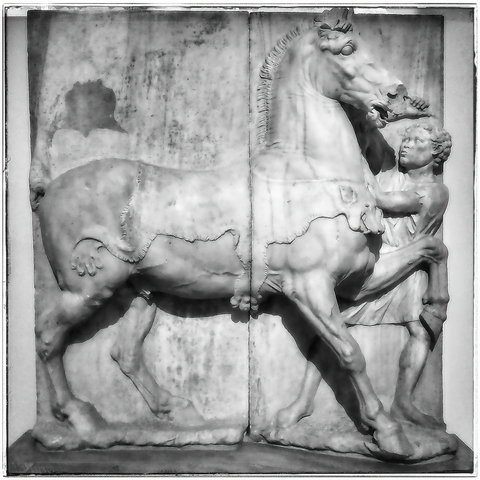
\includegraphics{smallthumb-lesson_I.jpeg}
\setfloatalignment{b}
\end{marginfigure}


\begin{abstract}
\noindent
Queste lezioni si articolano in \textsc{elementi grammaticali}, 
espressi sommariamente, seguiti da \textsc{vocabolari} per il lessico di base 
e da \textsc{frasi da tradurre} dal greco e in greco. 
\
L'approccio è quello del testo-laboratorio di morfosintassi: 
si presenta punto per punto - riprendendone la numerazione - 
l'esposizione di Gleason\cite{gleason1903}.\\
\bigskip
\noindent
Lezione IX: Perfetto e Piuccheperfetto indicativo attivo, il raddoppiamento, vocabolario, esercizi.
\end{abstract}

%\printclassoptions

\newthought{122.} Il tempi verbali perfetto e il piuccheperfetto presentano il raddoppiamento, che indica un'azione compiuta\sidenote{il raddoppiamento si trova in tutti i modi verbali, mentre l'aumento si trova solo all'indicativo}.

\newthought{123.} Nella maggior parte dei verbi che iniziano \textit{con una singola consonante,} il raddoppiamento avviene mettendo come prefisso quella stessa consonante, seguita da \textbf{ε,} come in \textbf{λύω,} perfetto \textbf{λέ-λυκα,} \textit{ho sciolto}. 
Ma se la consonante è una muta aspra (\textbf{φ, χ, θ}) per prefisso si prende la muta dolce corrispondente
\sidenote{\textbf{φ} $\rightarrow$ \textbf{π;} \textbf{χ} $\rightarrow$ \textbf{κ;} \textbf{θ} $\rightarrow$ \textbf{τ,}} 
come in \textbf{θύω,} perfetto \textbf{τέ-θυκα,} \textit{ho sacrificato}.

\newthought{124.} I verbi che iniziano \textit{con due consonanti\sidenote{eccetto si tratti di una muta seguita da una liquida (\textbf{λ, μ, ν, ρ}).}, con una consonante doppia o con \textbf{ρ,}} presentano aumento sillabico al posto del raddoppiamento, 
come in \textbf{ζητέω,} \textit{cercare,} perfetto \textbf{ἐ-ζήτηκα;}
\textbf{στρατεύω,} \textit{fare una spedizione,} perfetto \textbf{ἐ-στράτεθκα;} 
fa eccezione \textbf{γράφω,} perfetto \textbf{γέ-γραφα;}.
\newthought{Osservazione}
\begin{itemize}
\item[\textsc{1.}] Tutti i verbi che iniziano per \textbf{ρ,} raddoppiano questa lettera nel prefisso dell'aumento sillabico, come in \textbf{ῥίπτω,} \textit{tirare,} perfetto \textbf{ἔρ-ριφα.}  
\end{itemize}

\newthought{125.} Per i verbi che iniziano \textit{con una vocale corta o un dittongo,} il raddoppiamento prende la forma dell'aumento temporale, come in \textbf{ἄγω,} perfetto \textbf{ἦχα} e in \textbf{οἰκέω,} \textit{vivere,} perfetto \textbf{ᾤκηκα.}

\newpage

\newthought{126. Il Piuccheperfetto.} Quando il perfetto ha il raddoppiamento (123.), il piuccheperfetto presenta l'aumento sillabico come prefisso al raddoppiamento, come in \textbf{λύω,} perfetto \textbf{λέ-λυκα,} piuccheperfetto \textbf{ἐ-λε-λυκη.} Negli altri casi il piuccheperfetto mantiene l'aumento del perfetto, come in \textbf{στρατεύω,} perfetto \textbf{ἐστράτευκα,} piuccheperfetto \textbf{ἐστρατεύκη.}

\newthought{127. Perfetto e Piuccheperfetto Indicativo Attivo di \textbf{λύω.}} 

\begin{fullwidth}
\begin{table}[!htbp]
  \centering
  \begin{tabular}{l l l}
    %\toprule
	\multicolumn{3}{c}{\textsc{sistema del perfetto}} \\
	& \textsc{Perfetto} & \textsc{Piuccheperfetto} \\
	& \textit{Ho sciolto} & \textit{Avevo sciolto} \\
    %\midrule
	\multicolumn{3}{c}{\textsc{singolare}} \\
    \textsc{1.} & \textbf{λέλυκα}   & \textbf{ἐλελύκη} \\
    \textsc{2.} & \textbf{λέλυκας}   & \textbf{ἐλελύκης} \\
    \textsc{3.} & \textbf{λέλυκε}   & \textbf{ἐλελύκει} \\
	\multicolumn{3}{c}{\textsc{plurale}}  \\
	\textsc{1.} & \textbf{λελύκαμεν}   & \textbf{ἐλελύκεμεν} \\
    \textsc{2.} & \textbf{λελύκατε}   & \textbf{ἐλελύκετε} \\
    \textsc{3.} & \textbf{λελύκασι}   & \textbf{ἐλελύκεσαν} \\
    %\bottomrule
  \end{tabular}
  \caption{λύω: perfetto e piuccheperfetto indicativo attivo}
  \label{tab:normaltab}
  %\zsavepos{pos:normaltab}
\end{table}
\end{fullwidth}

\newthought{Esercizi}
\begin{itemize}
\item[\textsc{1.}] Coniuga allo stesso modo questi tempi per i verbi \textbf{θύω, κελεύω, παίω, θηρεύω,} e \textbf{κωλύω,} \textit{ostacolare.}  
\end{itemize}

\newthought{128. Vocabolario}

\begin{multicols}{2}
    \noindent \hangindent=1em \textbf{δείλη, ἡ} \textit{sera, pomeriggio}.  \\
    \noindent \hangindent=1em \textbf{κόρη, ἡ} \textit{ragazza}.  \\
    \noindent \hangindent=1em \textbf{νῆσος, ἡ} \textit{isola}.  \\
    \noindent \hangindent=1em \textbf{μεστός, ή, όν} agg. \textit{pieno di}.  \\
    \noindent \hangindent=1em \textbf{στενός, ή, όν} agg. \textit{stretto}.  \\

    \noindent \hangindent=1em \textbf{κωλύω,} fut. \textbf{κωλύσω,} aor. \textbf{ἐκώλυσα,} 
	pf. \textbf{κεκώλυσα,} 
	\textit{ostacolare, prevenire.} \\ 
	\noindent \hangindent=1em \textbf{στρατεύω,} fut. \textbf{στρατεύσω,} aor. \textbf{ἐστράτευσα,} 
	pf. \textbf{ἐστράτευκα,} 
	\textit{fare una spedizione, scendere in campo.} \\ 
	\noindent \hangindent=1em \textbf{ἐπεί,} avv. \textit{quando, dopo.} \\ 
	\noindent \hangindent=1em \textbf{εὐθύς,} avv. \textit{subito, immediatamente.} \\ 

	\noindent \hangindent=1em \textbf{παρά,} prep. 
	con \gen \textit{da, dal lato di}; 
	con \dat \textit{vicino a, al lato di}; 
	con \acc \textit{a, verso il lato di}.
	
\end{multicols}

\newthought{119. Traduci:}
\textsc{1.}~ἐλελύκεσαν, κεκελεύκασι, τέθυκας. \quad
\textsc{2.}~ἔλυσαν, πέπαικε, κεκωλύκαμεν. \quad
\textsc{3.}~λύε, ἔλυε, λύσει, ἔλυσε, λέλυκε, ἐλελύκει. \\
\textit{(a).} Scrivere, per il verbo θύω, tutti i tempi dell'indicativo alla terza persona plurale.

\newthought{130.}
\textsc{1.}~ὁ τῆς κόρης ἀδελφὸς εἶχε πλοῖοω καλόν. \quad
\textsc{2.}~τῷ δὲ τῆς κόρης ἀδελφῷ πλοῖον ἦν καλόν. \quad
\textsc{3.}~ἐν δὲ τῷ πλοίῳ ἤγαγε τὰ παιδία εἰς τὴν νῆσον. \quad
\textsc{4.}~ἡ γὰρ νῆσος μικρὰ ἦν, μεστὴ δὲ δένδρων μακρῶν καὶ καλῶν. \quad
\textsc{5.}~ἐπεὶ δὲ ὁ ἄγγελος ἐτεθύκει, ἐθήρευεν ἐν τῷ πεδίῳ. \quad
\textsc{6.}~καὶ εὐθὺς ἐδίωξε τὰ θηρία ἐκ τοῦ χωρίου. \quad
\textsc{7.}~ἡ δὲ βασίλεια κεκώλυκε αὐτὸν (suo) πέμπειν ἐπιστολὰ τῷ υἱῷ. \quad
\textsc{8.}~ἐπεὶ δείλη ἦν, ταχέως εἰς τὸν ποταμὸν ἔβαλον τοὺς βίκους μεστοὺς οἴνου. \quad
\textsc{9.}~εὐθὺς δὲ γράψουσι δικαίους λόγους. \quad
\textsc{10.}~τίς γὰρ ἔλιπεν ἐν ταῖς σκηναῖς τὰς λόγχας καὶ τὰς μαχαίρας;

\newthought{131. Scrivi in Greco:}
\textsc{1.}~Trovarono nel mare celle conchiglie.\quad
\textsc{2.}~Rimasero\sidenote{usa l'imperfetto.} cinque giorni nella casa \quad
\textsc{3.}~Vi erano cavalli e carri sul ponte. \quad
\textsc{4.}~La strada per l'altura era lunga.

\newthought{132. Sicuro di essere Grande:} Ἔλεγε δὲ τῷ Θεμιστοκλεῖ ὁ διδάσκαλος, Οὐδὲν ἔσῃ, παῖ, σὺ μικρόν, ἀλλά μέγα πάντως ἀγαθὸν ἢ (oppure) καλόν.

\begin{figure*}[!b]
  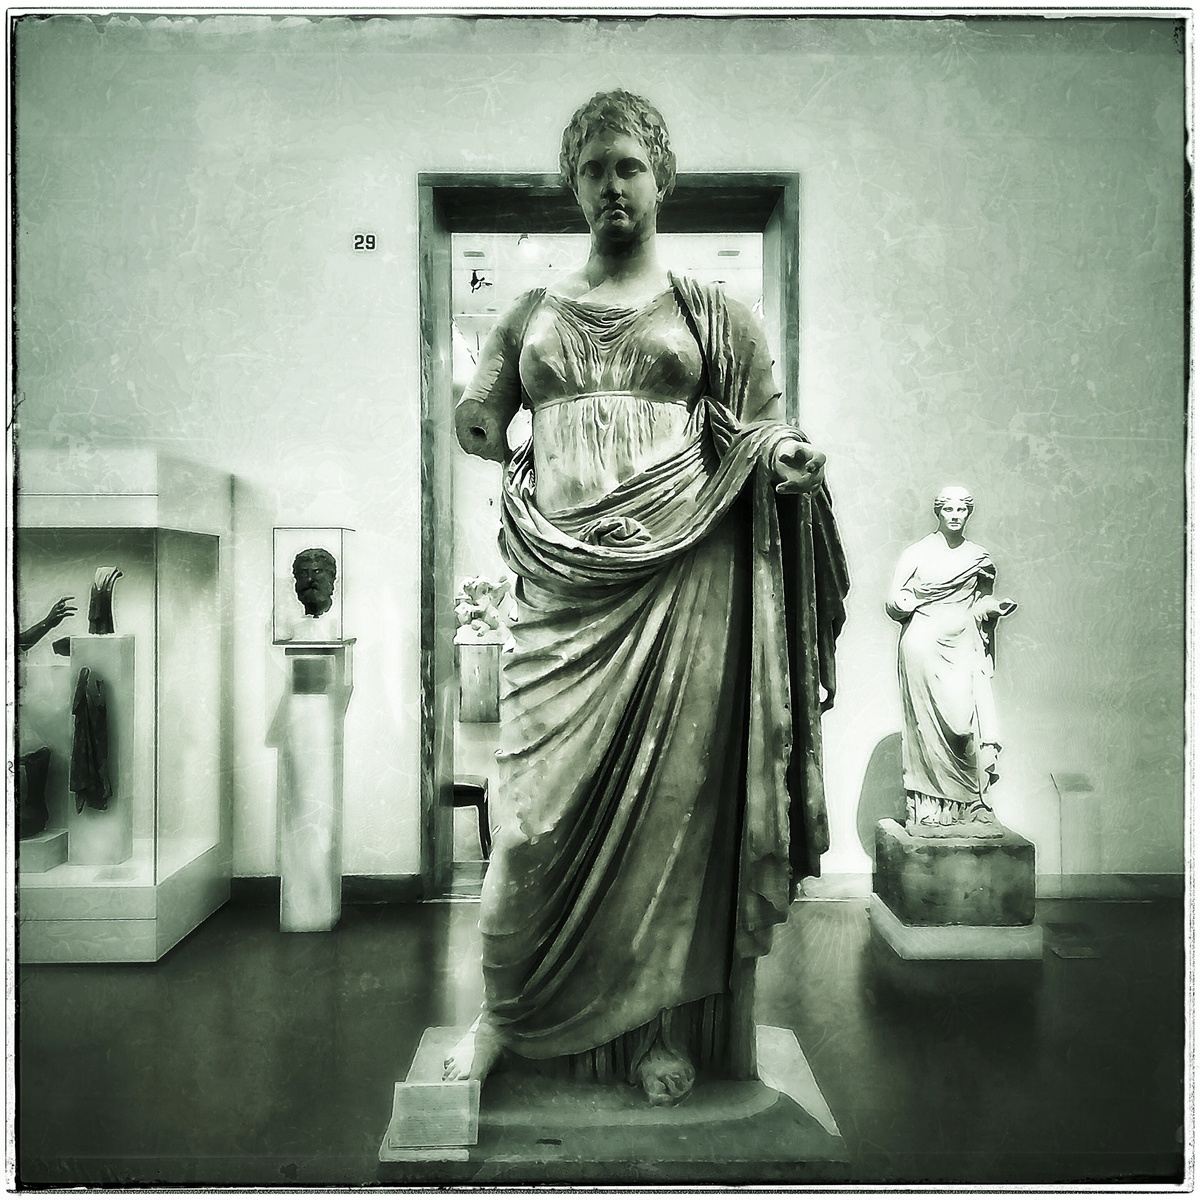
\includegraphics[width=0.7\linewidth]{thumb-lesson_X.jpeg}
  %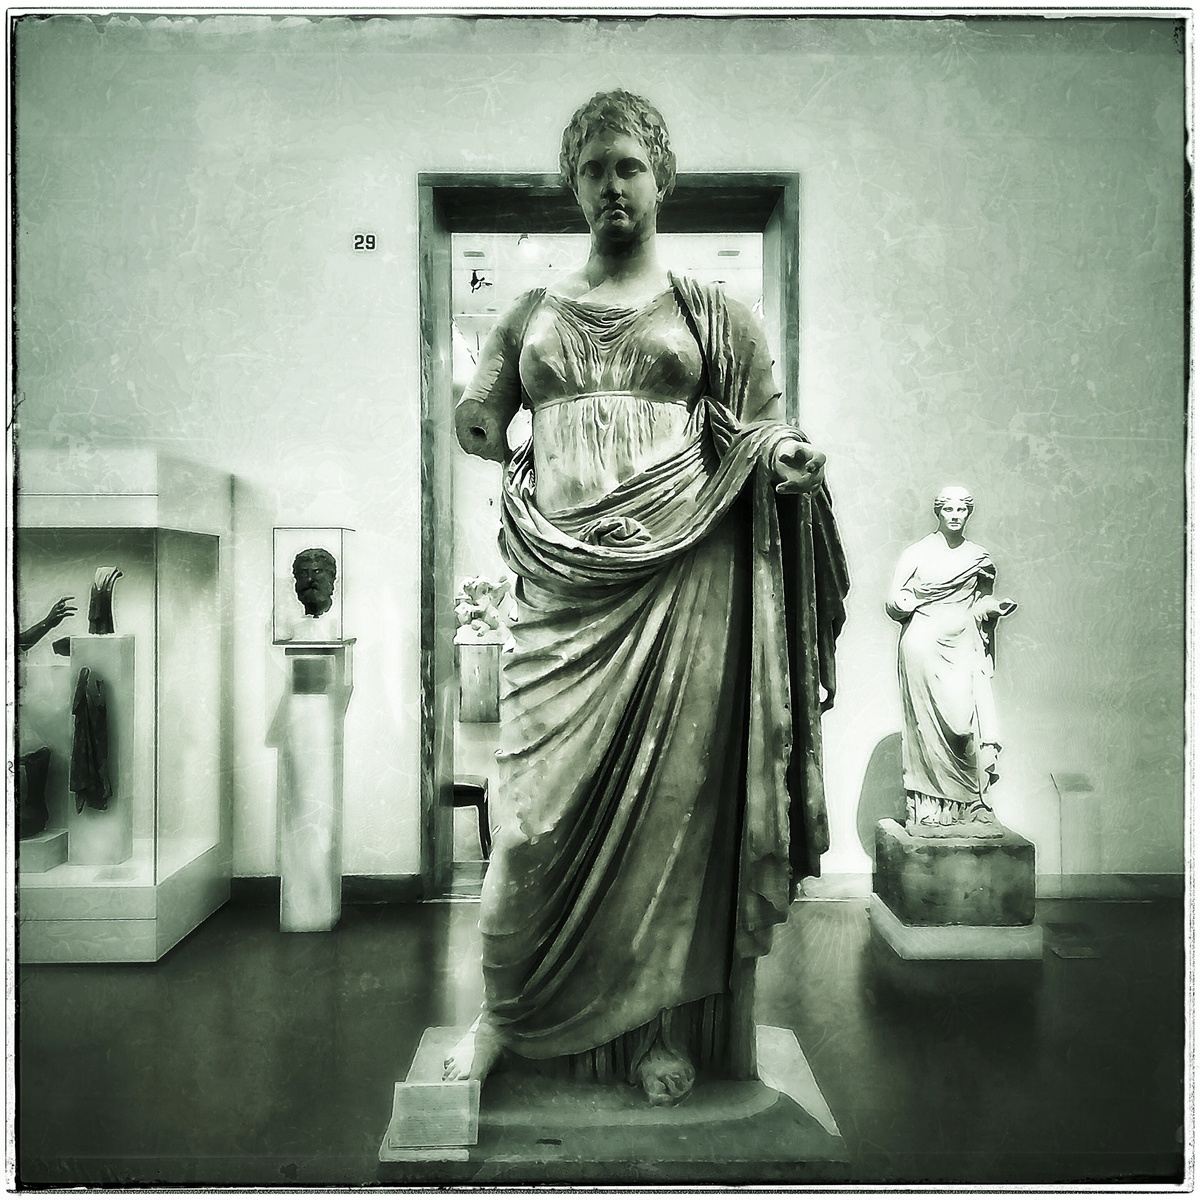
\includegraphics{thumb-lesson_X.jpeg}
  \caption{Museo Nazionale di Archeologia di Atene}
  \label{fig:textfig}
  %\zsavepos{pos:textfig}
  %\setfloatalignment{b}
\end{figure*}

 

\nobibliography{greekBiblio}
\bibliographystyle{alpha}


\end{document}
